\chapter{Monte Carlo lượng tử: giải bằng ngẫu nhiên}
\label{ch:qmc}

Các chương trước đều \emph{viết} hàm sóng ra dưới dạng tổ hợp các hàm cơ sở, và đều gặp bức tường tổ hợp hoặc phải xấp xỉ. Monte Carlo lượng tử (QMC) đi một con đường khác: \emph{không lưu hàm sóng}, mà chỉ lấy mẫu những cấu hình electron ``điển hình'' một cách ngẫu nhiên. Phương pháp này làm việc trực tiếp với tọa độ thật của electron, không cần tập cơ sở, và có thể dùng hàm sóng chứa $r_{12}$ tường minh.

\section{Ý tưởng Monte Carlo}

\begin{eli5}[đo diện tích hồ bằng cách ném đá]
Muốn đo diện tích một cái hồ có hình thù kỳ quặc nằm trong một mảnh đất hình vuông, bạn ném thật nhiều viên đá ngẫu nhiên vào mảnh đất và đếm tỉ lệ viên rơi xuống nước. Tỉ lệ đó nhân với diện tích mảnh đất cho diện tích hồ. Ném càng nhiều, kết quả càng chính xác.

Điều kỳ diệu: sai số chỉ phụ thuộc vào \emph{số viên đá}, không phụ thuộc vào \emph{số chiều} của ``mảnh đất''. Hàm sóng Li sống trong 9 chiều, Fe trong 78 chiều, nhưng sai số Monte Carlo vẫn giảm như $1/\sqrt{\text{số mẫu}}$. Đây chính là cách đi vòng qua bức tường hàm mũ.

\emph{Chỗ ví dụ ``gãy'':} ném đá \emph{đều} khắp nơi rất lãng phí khi hàm sóng chỉ lớn ở một vùng nhỏ. QMC ném đá \emph{thông minh}: nhiều hơn ở chỗ electron hay có mặt.
\end{eli5}

\begin{congthuc}[sai số Monte Carlo]
Trung bình của $M$ mẫu ngẫu nhiên độc lập có sai số chuẩn
\[
\sigma_{\bar x}=\frac{\sigma}{\sqrt M},
\]
với $\sigma$ là độ lệch chuẩn của một mẫu. Muốn giảm sai số 10 lần phải tăng số mẫu 100 lần, nhưng con số này \emph{không phụ thuộc số chiều} của tích phân. Với lưới đều trong $d$ chiều, sai số giảm như $M^{-k/d}$ (với $k$ là bậc chính xác của quy tắc tích phân), nên lưới hoàn toàn vô dụng khi $d$ lớn.
\end{congthuc}

\section{Monte Carlo biến phân (VMC)}

\begin{congthuc}[năng lượng như một trung bình]
Với hàm thử $\Psi_T(\mathbf R)$, trong đó $\mathbf R=(\vr_1,\vr_2,\vr_3)$ là vị trí cả ba electron, năng lượng biến phân viết được thành
\[
E[\Psi_T]=\frac{\int|\Psi_T(\mathbf R)|^2\,E_L(\mathbf R)\,d\mathbf R}{\int|\Psi_T(\mathbf R)|^2\,d\mathbf R},\qquad
E_L(\mathbf R)=\frac{\Hhat\Psi_T(\mathbf R)}{\Psi_T(\mathbf R)} .
\]
\begin{itemize}
\item $|\Psi_T|^2/\!\int|\Psi_T|^2$ là một \textbf{phân bố xác suất} trên không gian 9 chiều: xác suất thấy ba electron ở ba vị trí $\vr_1,\vr_2,\vr_3$.
\item $E_L$ là \textbf{năng lượng cục bộ} \en{local energy}: một con số tính được tại từng cấu hình $\mathbf R$.
\item Vậy $E$ chỉ là \emph{trung bình} của $E_L$ trên các cấu hình lấy mẫu theo $|\Psi_T|^2$: $E\approx\frac1M\sum_{k=1}^M E_L(\mathbf R_k)$.
\end{itemize}
\textbf{Tính chất ``phương sai bằng không'':} nếu $\Psi_T$ là hàm sóng chính xác thì $\Hhat\Psi_T=E_0\Psi_T$, nên $E_L(\mathbf R)=E_0$ \emph{tại mọi điểm}. Mọi mẫu cho cùng một giá trị và sai số thống kê bằng 0. Hàm thử càng tốt, $E_L$ càng ít dao động. Đây là một ``đồng hồ đo chất lượng'' rất hữu ích.
\end{congthuc}

\subsection{Thuật toán Metropolis}
Làm sao lấy mẫu theo một phân bố 9 chiều phức tạp như $|\Psi_T|^2$? Thuật toán Metropolis (1953) \cite{Metropolis1953} cho một ``người đi bộ ngẫu nhiên'' \en{walker} đi lang thang sao cho lâu dần, thời gian nó ở mỗi vùng tỉ lệ với $|\Psi_T|^2$:
\begin{enumerate}
\item Từ cấu hình hiện tại $\mathbf R$, đề xuất bước mới $\mathbf R'=\mathbf R+\boldsymbol\delta$ ($\boldsymbol\delta$ ngẫu nhiên nhỏ).
\item Chấp nhận bước với xác suất $\min\!\big(1,\,|\Psi_T(\mathbf R')|^2/|\Psi_T(\mathbf R)|^2\big)$; nếu không chấp nhận thì đứng yên.
\item Lặp lại. Sau một thời gian ``làm nóng'', các cấu hình là mẫu của $|\Psi_T|^2$.
\end{enumerate}
Điểm hay: chỉ cần \emph{tỉ số} $\Psi_T(\mathbf R')/\Psi_T(\mathbf R)$, không cần biết hằng số chuẩn hóa (một tích phân 9 chiều mà ta không tính được).

\begin{figure}[h]
\centering
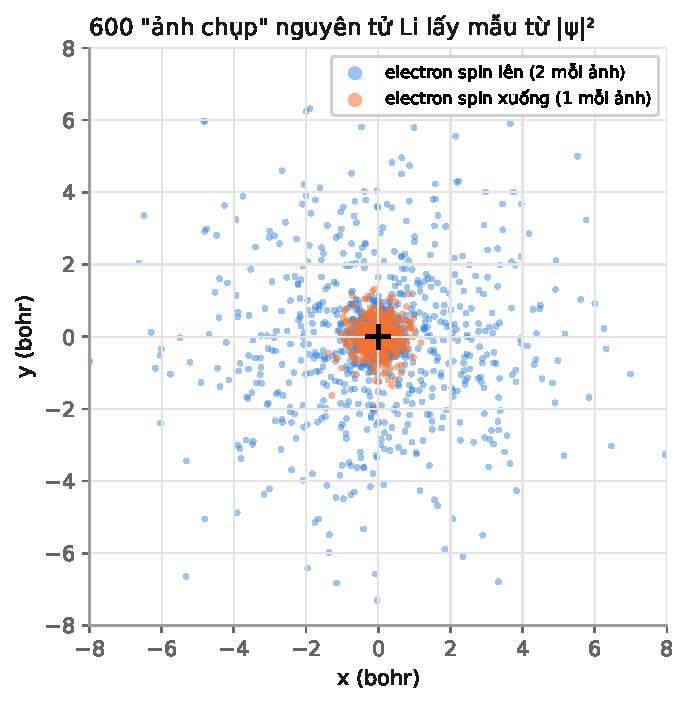
\includegraphics[width=0.6\textwidth]{05_dam_may_electron.pdf}
\caption{600 ``ảnh chụp'' nguyên tử Li do thuật toán Metropolis lấy mẫu từ $|\Psi_T|^2$ (chiếu xuống mặt phẳng $xy$). Mỗi ảnh có 2 electron spin lên (xanh) và 1 electron spin xuống (cam). Electron spin xuống hầu như luôn ở lớp trong; hai electron spin lên thường có một ở lớp trong và một ở lớp ngoài: đúng bức tranh 1s$^2$2s. (Script \code{05\_monte\_carlo\_luong\_tu.py})}
\label{fig:dammay}
\end{figure}

\subsection{Hàm thử Slater--Jastrow}
Hàm thử phổ biến nhất trong QMC là \textbf{định thức Slater nhân thừa số Jastrow} \cite{Jastrow1955}:
\[
\Psi_T(\mathbf R)=D_\uparrow(\vr_1,\vr_2)\,D_\downarrow(\vr_3)\,e^{J(\mathbf R)} .
\]
Phần định thức lo việc phản đối xứng (và nguyên lý Pauli). Phần Jastrow $e^J$ luôn dương, nên không làm thay đổi dấu của hàm sóng, nhưng mô tả việc các electron ``né nhau''. Đây đúng là thứ Hartree--Fock thiếu.

\begin{congthuc}[hàm thử dùng trong code]
\begin{itemize}
\item Orbital: $\phi_1(r)=e^{-z_1r}$ (kiểu 1s) và $\phi_2(r)=(1-cr)e^{-z_2r}$ (kiểu 2s, có một nút), với $c=z_1-z_2$.
\item Định thức spin lên: $D_\uparrow=\phi_1(r_1)\phi_2(r_2)-\phi_1(r_2)\phi_2(r_1)$. Spin xuống: $D_\downarrow=\phi_1(r_3)$.
\item Jastrow electron--electron: $J_{ee}=\sum_{i<j}\dfrac{a_{ij}\,r_{ij}}{1+b\,r_{ij}}$, với $a_{ij}=\tfrac12$ cho cặp ngược spin và $\tfrac14$ cho cặp cùng spin. Khi $r_{ij}\to0$, $e^{J}\approx1+a_{ij}r_{ij}$: đúng điều kiện cusp của Kato (mục~\ref{sec:cusp}).
\item Jastrow electron--hạt nhân: $J_{en}=-\sum_i\dfrac{(Z-z_1)\,r_i}{1+d\,r_i}$. Cộng với đạo hàm của orbital tại gốc ($-z_1$), đạo hàm log của $\Psi_T$ khi electron chạm hạt nhân đúng bằng $-Z$: thỏa cusp electron--hạt nhân.
\end{itemize}
Bốn tham số $(z_1,z_2,d,b)$ được tối ưu để năng lượng nhỏ nhất. Gradient và laplacian của $\Psi_T$ (cần cho $E_L$) được tính bằng công thức giải tích và kiểm tra lại bằng sai phân hữu hạn (khớp tới $10^{-7}$).
\end{congthuc}

\begin{hieulam}[bỏ qua điều kiện cusp]
Phiên bản đầu tiên của code \emph{không} thỏa điều kiện cusp electron--hạt nhân. VMC vẫn chạy được, nhưng năng lượng cục bộ $E_L$ tiến ra vô cùng mỗi khi một electron tới sát hạt nhân. Với DMC (mục sau), điều này làm quần thể walker ``bùng nổ'' và cho năng lượng $-50\Ha$, một con số vô nghĩa. Điều kiện cusp không phải chi tiết toán học cho đẹp: nó quyết định phương pháp có chạy được hay không.
\end{hieulam}

Kết quả VMC (bảng~\ref{tab:qmc}): chỉ dùng định thức Slater với các orbital đơn giản chưa tối ưu, $E=\EvmcSlater\Ha$, còn cao hơn cả giới hạn Hartree--Fock. Thêm Jastrow và tối ưu 4 tham số, $E=\Evmc\Ha$, thu \PctVmc\% năng lượng tương quan, chỉ với 4 tham số. Để so sánh: Full CI cần gần 300\,000 định thức mới thu được khoảng 96\%.

\section{Monte Carlo khuếch tán (DMC)}

VMC chỉ tốt bằng hàm thử. DMC đi xa hơn: nó \emph{tự động} lọc hàm thử để tiến về trạng thái cơ bản thật.

\begin{eli5}[mực loang trong nước]
Thay $t$ trong phương trình Schrödinger phụ thuộc thời gian bằng ``thời gian ảo'' $\tau=it$. Phương trình trở thành giống phương trình \emph{khuếch tán}, mô tả mực loang trong nước, cộng thêm một số hạng ``sinh--diệt''. Thả một đám walker; mỗi walker khuếch tán ngẫu nhiên. Walker ở vùng thế năng thấp (gần hạt nhân) thì ``sinh sôi'' (nhân bản), walker ở vùng thế năng cao thì ``chết'' (biến mất). Sau đủ lâu, đám walker phân bố đúng theo hàm sóng của trạng thái cơ bản, bất kể ban đầu thả thế nào.
\end{eli5}

\begin{congthuc}[phép chiếu bằng thời gian ảo]
Khai triển hàm ban đầu theo các trạng thái riêng, $\Psi(0)=\sum_n c_n\Psi_n$, rồi ``tiến hóa'' theo thời gian ảo:
\[
\Psi(\tau)=e^{-(\Hhat-E_T)\tau}\Psi(0)=\sum_n c_n\,e^{-(E_n-E_T)\tau}\,\Psi_n
\;\xrightarrow{\tau\to\infty}\;c_0\,e^{-(E_0-E_T)\tau}\,\Psi_0 .
\]
Mọi trạng thái kích thích tắt dần theo $e^{-(E_n-E_0)\tau}$ nhanh hơn trạng thái cơ bản, nên chỉ còn lại $\Psi_0$. Năng lượng thử $E_T$ được điều chỉnh liên tục để giữ số walker ổn định. Phương trình tương ứng
\[
-\frac{\partial\Psi}{\partial\tau}=-\tfrac12\nabla^2\Psi+(V-E_T)\Psi
\]
có hai phần: $-\tfrac12\nabla^2$ là khuếch tán (walker đi ngẫu nhiên), $(V-E_T)$ là sinh--diệt (walker nhân bản hay biến mất với trọng số $e^{-(V-E_T)\delta\tau}$). Thực tế người ta dùng \textbf{lấy mẫu theo tầm quan trọng} \en{importance sampling}: walker còn ``trôi'' theo vận tốc $\nabla\ln|\Psi_T|$ về phía hàm thử lớn, và trọng số dùng $E_L$ thay cho $V$, nên dao động nhỏ hơn rất nhiều \cite{Reynolds1982,Umrigar1993}.
\end{congthuc}

\section{Bài toán dấu và gần đúng nút cố định}

DMC coi hàm sóng như \emph{mật độ} của walker, mà mật độ thì không âm. Nhưng hàm sóng fermion bắt buộc đổi dấu (phản đối xứng)! Nếu cứ để walker tự do, đám walker sẽ hội tụ về trạng thái thấp nhất \emph{không có ràng buộc đối xứng}, tức là ``trạng thái boson'', như cái bẫy boson ở hình~\ref{fig:bacthang}.

\begin{eli5}[cộng những số khổng lồ trái dấu]
Muốn tính một con số nhỏ bằng cách cộng hàng triệu số dương khổng lồ với hàng triệu số âm khổng lồ gần bằng chúng: chỉ một sai số nhỏ trong mỗi số cũng làm kết quả cuối cùng vô nghĩa. Mô phỏng fermion bằng walker mang dấu $+$ và $-$ gặp đúng tình trạng này: tín hiệu (hiệu của hai đám walker) tắt dần theo hàm mũ, còn nhiễu thì không. Đó là \textbf{bài toán dấu} \en{sign problem}.
\end{eli5}

Troyer và Wiese (2005) đã chứng minh rằng một lời giải tổng quát cho bài toán dấu sẽ kéo theo việc giải được cả lớp bài toán NP-khó \cite{TroyerWiese2005}, nên khó có hy vọng tìm ra ``thuốc chữa'' tổng quát. Cách làm thực tế là \textbf{gần đúng nút cố định} \en{fixed-node approximation} \cite{Reynolds1982}: lấy \emph{nút} (mặt $\Psi_T=0$) của hàm thử làm ``tường'', cấm walker đi xuyên qua. Trong mỗi vùng kẹp giữa các nút, hàm sóng không đổi dấu nên DMC chạy bình thường. Kết quả là năng lượng thấp nhất có cùng mặt nút với $\Psi_T$. Đây vẫn là một cận trên biến phân: nếu nút đúng thì năng lượng đúng, nếu nút sai thì năng lượng cao hơn một chút.

Với hàm thử của chúng ta, nút có dạng rất đơn giản. $D_\uparrow=0$ khi $\phi_2(r_1)/\phi_1(r_1)=\phi_2(r_2)/\phi_1(r_2)$. Vì tỉ số $\phi_2/\phi_1=(1-cr)e^{(z_1-z_2)r}$ là hàm giảm đơn điệu theo $r$ (có thể kiểm tra bằng đạo hàm), nút chính là mặt $r_1=r_2$: \emph{hai electron cùng spin cách hạt nhân bằng nhau}. Đây cũng chính là nút của hàm Hartree--Fock, và các nghiên cứu cho thấy nó trùng gần như hoàn toàn với nút của hàm sóng chính xác \cite{Bressanini2001,Brown2007}. (Với Be, chỉ thêm một electron, nút của Hartree--Fock đã sai về hình dạng tô-pô và gây sai số khoảng $10\mHa$.)

\section{Kết quả cho Li}

\begin{chaycode}[QMC trong 300 dòng numpy]
Script \code{05\_monte\_carlo\_luong\_tu.py} cài đặt VMC (Metropolis, tối ưu tham số bằng lấy mẫu tương quan) và DMC (lấy mẫu theo tầm quan trọng, chấp nhận Metropolis--Hastings, nút cố định, giới hạn vận tốc trôi theo Umrigar và cộng sự \cite{Umrigar1993}) với 4000 walker. DMC chạy với 4 bước thời gian $\tau$ khác nhau rồi ngoại suy về $\tau\to0$, vì phép chia thời gian thành các bước hữu hạn gây ra một sai số hệ thống tỉ lệ với $\tau$.
\end{chaycode}

\begin{table}[h]
\centering\small
\caption{Kết quả Monte Carlo lượng tử tự viết cho Li (script \code{05\_monte\_carlo\_luong\_tu.py}). Sai số thống kê ($1\sigma$) ghi sau dấu $\pm$.}
\label{tab:qmc}
\begin{tabular}{@{}lrrr@{}}
\toprule
Phương pháp & $E$ (Ha) & $E-E_{\text{chính xác}}$ (mHa) & \% tương quan \\
\midrule
VMC, chỉ định thức Slater & $-7.4182\pm0.0017$ & $+59.9$ & -32\% \\
VMC, Slater--Jastrow tối ưu & $-7.47444\pm0.00021$ & $+3.63$ & 92.0\% \\
DMC, $\tau=0.04$ & $-7.47918\pm0.00010$ & $-1.12$ & 102.5\% \\
DMC, $\tau=0.02$ & $-7.47834\pm0.00009$ & $-0.28$ & 100.6\% \\
DMC, $\tau=0.01$ & $-7.47804\pm0.00009$ & $+0.02$ & 100.0\% \\
DMC, $\tau=0.005$ & $-7.47818\pm0.00008$ & $-0.12$ & 100.3\% \\
DMC, ngoại suy $\tau\to0$ & $-7.47787\pm0.00007$ & $+0.19$ & 99.6\% \\
\midrule
Chính xác & $-7.47806$ & 0 & 100\% \\
\bottomrule
\end{tabular}
\end{table}


\begin{figure}[h]
\centering
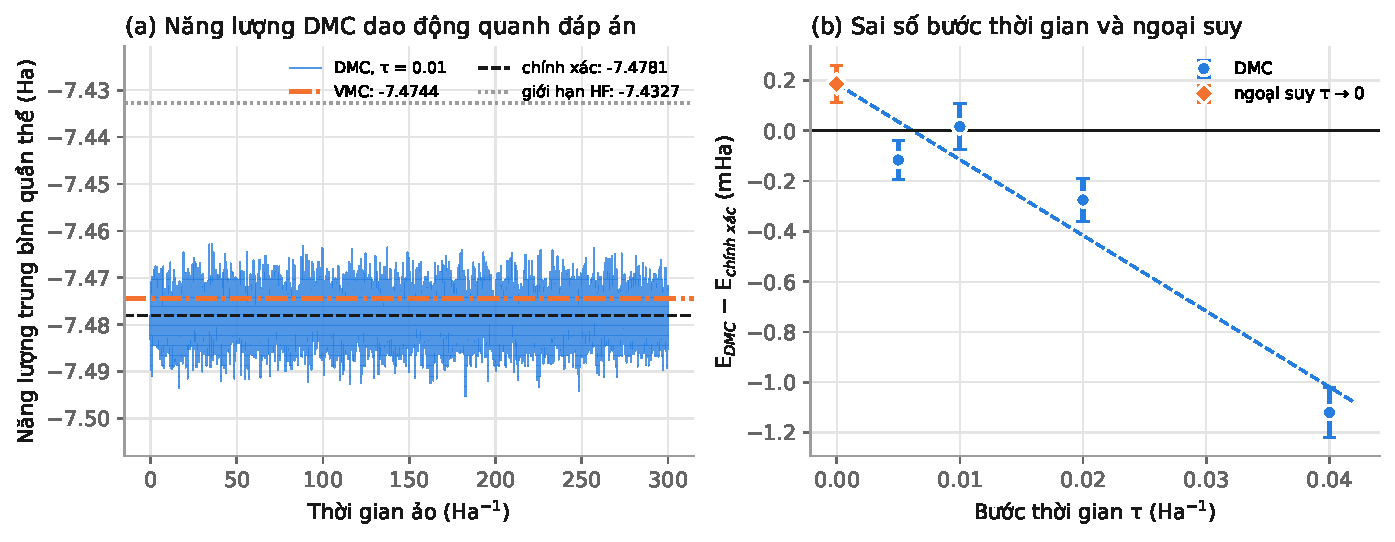
\includegraphics[width=\textwidth]{05_qmc_li.pdf}
\caption{(a) Năng lượng trung bình của quần thể walker DMC theo thời gian ảo ($\tau=0.01$): dao động thống kê quanh năng lượng chính xác (vạch đen), thấp hơn hẳn VMC (vạch cam) và giới hạn HF (vạch xám). (b) Năng lượng DMC theo bước thời gian $\tau$; đường nét đứt là ngoại suy tuyến tính về $\tau\to0$. (Script \code{05\_monte\_carlo\_luong\_tu.py})}
\label{fig:qmc}
\end{figure}

DMC ngoại suy về $\tau\to0$ cho $E=\Edmc\Ha$, tức lệch $\ErrDmc\mHa$ so với đáp án, với sai số thống kê $\pm\EdmcErr\mHa$. Ta thu được khoảng \PctDmc\% năng lượng tương quan bằng một chương trình vài trăm dòng, không cần tập cơ sở, với một hàm thử chỉ có 4 tham số. Đây là sức mạnh của QMC.

Cần nói thật một điều: độ lệch $\ErrDmc\mHa$ lớn hơn vài lần sai số thống kê ước tính, nên không thể coi hoàn toàn là nhiễu ngẫu nhiên. Có thể so với tài liệu: DMC chuyên nghiệp dùng \emph{đúng} mặt nút $r_1=r_2$ này (nút của hàm Hartree--Fock \cite{Bressanini2001}) cho $-7.47802(1)\Ha$, chỉ cao hơn đáp án $0.04\mHa$ \cite{Brown2007}. Vậy phần lớn độ lệch còn lại của ta \emph{không} do mặt nút, mà do cách cài đặt đơn giản: sai số bước thời gian chưa được khử hết (hình~\ref{fig:qmc}b cho thấy hai điểm có $\tau$ nhỏ nhất không thẳng hàng hoàn hảo), sai lệch nhỏ do cơ chế điều khiển số walker, và sai số thống kê bị ước tính hơi thấp vì các bước liên tiếp tương quan với nhau. Tách bạch các nguồn này là một bài tập hay cho người đọc. Dù vậy, sai số cỡ $0.2\mHa$ vẫn nhỏ hơn độ chính xác hóa học khoảng 8 lần.

\begin{table}[h]
\centering\small
\caption{So sánh với các kết quả QMC đã công bố cho Li.}
\label{tab:qmclit}
\begin{tabular}{@{}lrr@{}}
\toprule
Tính toán & $E$ (Ha) & \% tương quan \\
\midrule
VMC, Slater--Jastrow, 4 tham số (code đi kèm) & $\Evmc$ & \PctVmc \\
VMC, Slater--Jastrow chuyên nghiệp \cite{Brown2007} & $-7.47683(3)$ & 97.3 \\
VMC, nhiều định thức + Jastrow + backflow \cite{Seth2011} & $-7.478034(8)$ & 99.94 \\
DMC, nút $r_1=r_2$ (code đi kèm, $\tau\to0$) & $\Edmc$ & \PctDmc \\
DMC, nút Hartree--Fock \cite{Brown2007} & $-7.47802(1)$ & 99.91 \\
FermiNet, mạng nơ-ron (chương~\ref{ch:biengioi}) \cite{Pfau2020} & $-7.47798(1)$ & 99.82 \\
\midrule
Chính xác (Hylleraas) & $-7.478060$ & 100 \\
\bottomrule
\end{tabular}
\end{table}

Cũng cần nhớ: với Li, nút $r_1=r_2$ gần như chính xác; với các phân tử phức tạp hơn, sai số nút cố định thường cỡ vài mHa và là giới hạn chính của DMC \cite{Foulkes2001}.

\section{Ưu và nhược điểm}
\begin{itemize}
\item \textbf{Ưu:} chi phí tăng như $N^3$--$N^4$ theo số electron (cho mỗi mẫu); không cần tập cơ sở; dùng được hàm sóng chứa $r_{ij}$; song song hóa gần như hoàn hảo (mỗi walker độc lập), rất hợp với siêu máy tính; DMC thường chính xác ngang CCSD(T).
\item \textbf{Nhược:} kết quả luôn có sai số thống kê, muốn giảm 10 lần phải chạy lâu 100 lần; sai số nút cố định khó kiểm soát; tính lực (đạo hàm năng lượng theo vị trí hạt nhân) và các tính chất khác ngoài năng lượng khó hơn nhiều; cần nhiều kinh nghiệm để chọn hàm thử tốt.
\end{itemize}

\begin{ghinho}
\begin{itemize}
\item Monte Carlo tính tích phân nhiều chiều với sai số $\sim1/\sqrt M$, không phụ thuộc số chiều: một cách đi vòng bức tường hàm mũ.
\item VMC: năng lượng là trung bình của năng lượng cục bộ $E_L=\Hhat\Psi_T/\Psi_T$ trên các cấu hình lấy mẫu từ $|\Psi_T|^2$ bằng thuật toán Metropolis. Hàm Slater--Jastrow với 4 tham số thu \PctVmc\% tương quan của Li.
\item DMC: tiến hóa theo thời gian ảo để chiếu về trạng thái cơ bản. Fermion gây ra bài toán dấu; gần đúng nút cố định giải quyết bằng cách cấm walker vượt nút của hàm thử.
\item Điều kiện cusp là bắt buộc để DMC ổn định. Code tự viết đạt sai số $\ErrDmc\mHa$ so với đáp án 15 chữ số.
\end{itemize}
\end{ghinho}
